
\chapter{Emotion Usage Relationship}
should write something here




\subsection{Demography of participants}
There were a total of 26 participants. 19 of them were male and 7 were female. Most of them were students and some are from other occupations. 
\begin{figure}
\centering
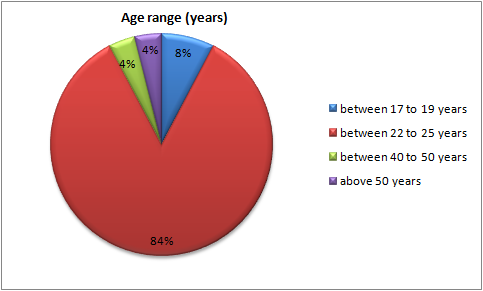
\includegraphics[width=1.75in,clip,keepaspectratio]{Chapters/figures/ageChart3}
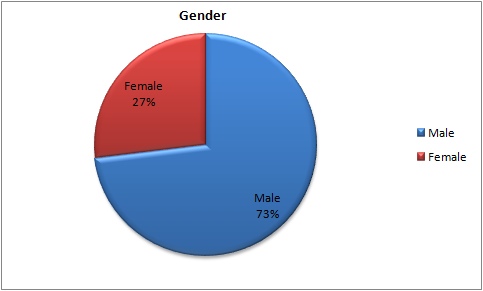
\includegraphics[width=1.75in,clip,keepaspectratio]{Chapters/figures/gender3}
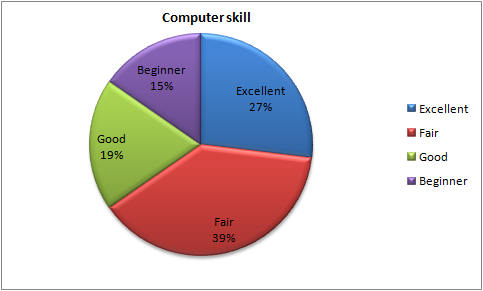
\includegraphics[width=1.75in,clip,keepaspectratio]{Chapters/figures/skill}
\caption{Category of users based on age range, gender, and computer operating skill}
\label{Optional 3 }
\end{figure}




\subsection{Classification methods}
\subsubsection{Bounded k-means clustering}
In these approach we used a variant of k-means clustering approach, where we put a constraint on the cluster size. The cluster size was varied to find out the optimal cluster size so that the total false acceptance and false rejection are minimized. The size was varied with percentages of mean and standard deviation.

\begin{figure}
\centering
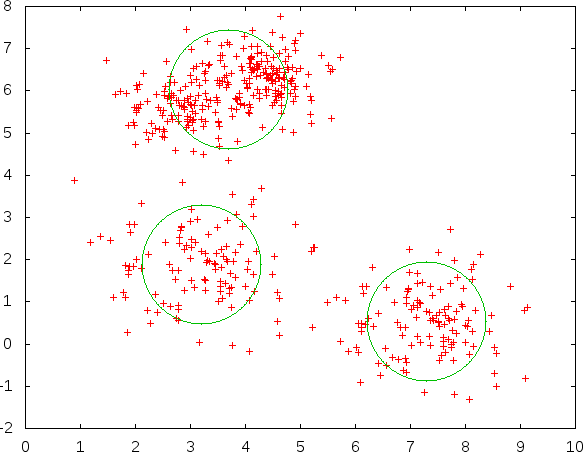
\includegraphics[width=3in,clip,keepaspectratio]{Chapters/figures/boundeKmeans}
\caption{bounded k-means clustering}
\label{Optional 4 }
\end{figure}

\subsubsection{k-nearest neighbor}
We used this well known classification method where a test point is classified by examining its neighbor points. We varied both the number of neighbors and the number of attributes.

\subsection{Identification of emotional states}
At first we tried to classify human emotions based on the usage attributes we captured in each step of the survey process. Every captured data is like the following format:
Att1, att2, att3, ………, emotion label, user label.

\subsubsection{10 classes of emotions}
We tried to classify 10 different emotional states. These are amusement, happiness, inspiration, surprise, sadness, sympathy, anger, disgust, fear and neutral emotion.
We tried two different classification approaches: bounded k-means clustering and k-nearest neighbor method.
\begin{center}
\begin{table}

\centering
\begin{tabular}{ |c|c|c| } 
 \hline
 method & false accept rate & false reject rate \\ 
 \hline
 bounded k-means & 0.43 & 0.34 \\ 
 knn & 0.76 & 0.0 \\ 
 \hline
\end{tabular}

\caption{bounded k-means and knn for 10 class emotion classification}
\label{table:1}
\end{table}
\end{center}

\begin{figure}
\centering
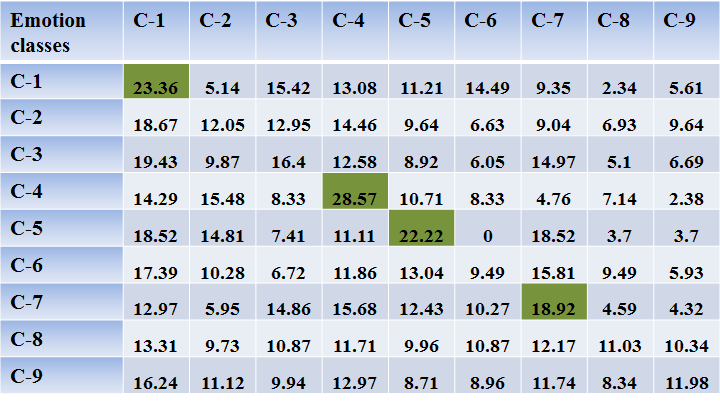
\includegraphics[width=4.25in,clip,keepaspectratio]{Chapters/figures/emotionMatrix}
\caption{Matrix of domination for 9-emotion classes(without the neutral emotion)}
\label{Optional 6}
\end{figure}


\begin{figure}
\centering
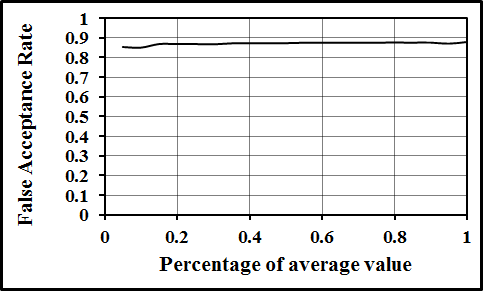
\includegraphics[width=2.5in,clip,keepaspectratio]{Chapters/figures/Emotion/10class/fA}
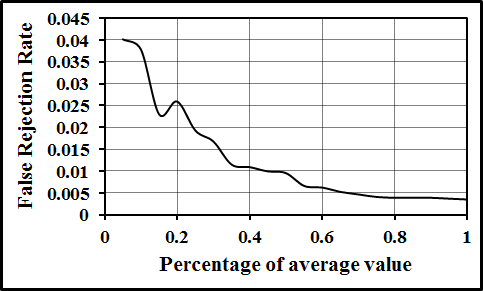
\includegraphics[width=2.5in,clip,keepaspectratio]{Chapters/figures/Emotion/10class/fR}
\caption{percentage of average vs false accept rate and false reject rate in bounded k-means for 10 class emotion classification}
\label{Optional 5}
\end{figure}

\begin{figure}
\centering
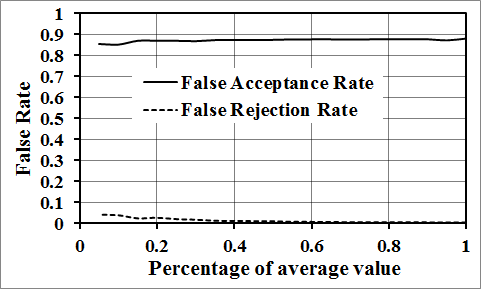
\includegraphics[width=4.25in,clip,keepaspectratio]{Chapters/figures/Emotion/10class/fAfR}
\caption{percentage of average vs false accept rate and false reject rate in bounded k-means for 10 class emotion classification}
\label{Optional 5}
\vskip -1cm
\end{figure}



\subsubsection{3 classes of emotions}
We grouped the 10 classes into 3 groups. The positive emotions such as amusement, happiness, inspiration and surprise were grouped into one class. The negative emotions such as sadness, sympathy, anger, disgust and fear were grouped into one class. Neutral emotion was considered as the third class.


\begin{center}
\begin{table}

\centering
\begin{tabular}{ |c|c|c| } 
 \hline
 method & false accept rate & false reject rate \\ 
 \hline
 bounded k-means & 0.25 & 0.17 \\ 
 knn & 0.47 & 0.0 \\ 
 \hline
\end{tabular}

\caption{bounded k-means and knn for 3 class emotion classification}
\label{table:2}
\end{table}
\end{center}


\begin{figure}
\centering
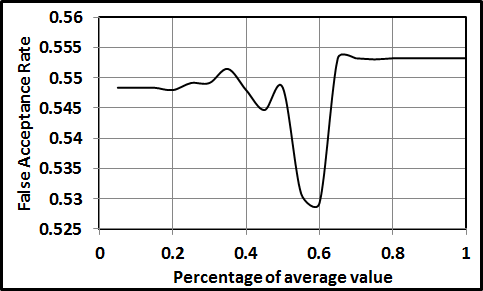
\includegraphics[width=4.25in,clip,keepaspectratio]{Chapters/figures/Emotion/3class/fA}
\caption{percentage of average vs false accept rate and false reject rate in bounded k-means for 3 class emotion classification}
\label{Optional 6}
\end{figure}


\clearpage
\subsubsection{Dominant classes of emotions}

\begin{center}

\begin{table}

\centering
\begin{tabular}{ |c|c|c|c|c| } 
 \hline
 classes & Amusement & Surprise & Sadness & Anger \\
\hline
Amusement & 36.31 &  25.34 &  16.75 &  21.60 \\ 
Surprise & 28.83 &  31.08 &  21.62 &  18.47 \\
Sadness & 27.60 &  25.04 &  22.78  & 24.59 \\ 
Anger & 24.04 &  22.70 &  18.43 &  34.83 \\

\hline
\end{tabular}

\caption{matrix of cluster with only dominant emotions}
\label{table:4}
\end{table}
\end{center}

\begin{figure}
\centering
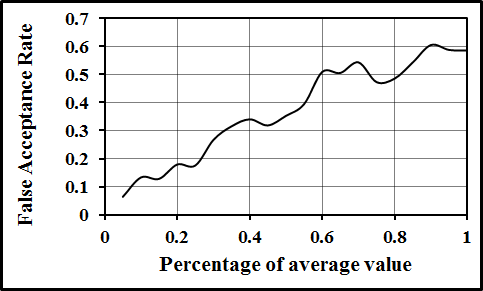
\includegraphics[width=2.5in,clip,keepaspectratio]{Chapters/figures/Emotion/dominant/fA}
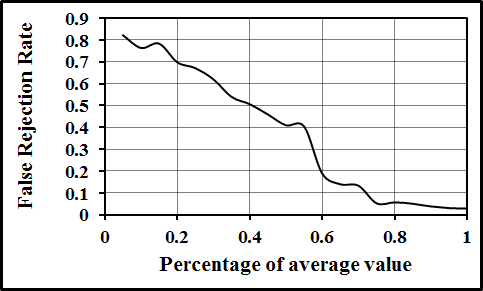
\includegraphics[width=2.5in,clip,keepaspectratio]{Chapters/figures/Emotion/dominant/fR}

\caption{percentage of average vs false accept rate and false reject rate in bounded k-means for dominant emotion classfication}
\label{Optional 6}
\end{figure}

\begin{figure}
\centering
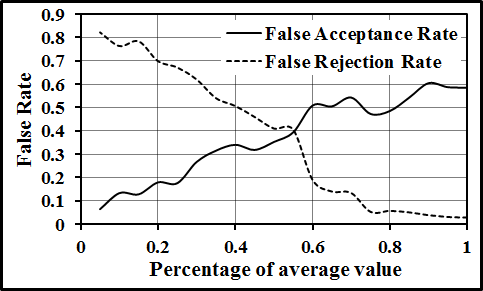
\includegraphics[width=4.25in,clip,keepaspectratio]{Chapters/figures/Emotion/dominant/fAfR}
\caption{percentage of average vs both false accept rate and false reject rate in bounded k-means for dominant emotion classfication}
\label{Optional 6}
\end{figure}


From the unsupervised bounded k-means clustering of 10 emotions. We found 10 different clusters, but this clusters were not dominated by only one class of emotion. Rather we found that there are some emotions which dominates not only in his own cluster but also in the clusters of others. While trying to classify these dominant clusters only we found some improvement. The experimental results are as followed from bounded k-means clustering and k-nearest neighbor classification:


\clearpage
\subsubsection{Less Dominant classes of emotions}
From the cluster matrix we can identify the clusters(emotions) which has less influence over their own clusters and others clusters. When we tried to classify these less dominant emotions, we found the following results:


\begin{table}

\centering
\begin{tabular}{ |c|c|c|c|c|c| } 
 \hline
 classes & c-1 & c-2 & c-3 & c-4 & c-5\\
\hline
c-1 & 26.32 & 26.32 & 16.67 & 12.72 & 17.98 \\
c-2 & 18.69 & 38.13 & 17.93 & 11.62 & 13.64 \\ 
c-3 & 21.31 & 21.31 & 26.23 & 17.49 & 13.66 \\
c-4  & 18.34 & 20.92 & 20.63 & 20.77 & 19.34 \\
c-5  & 22.09 & 19.75 & 17.79 & 16.56 & 23.80 \\

\hline
\end{tabular}

\caption{matrix of cluster with less dominant emotions}
\label{table:5}
\end{table}


\begin{figure}
\centering
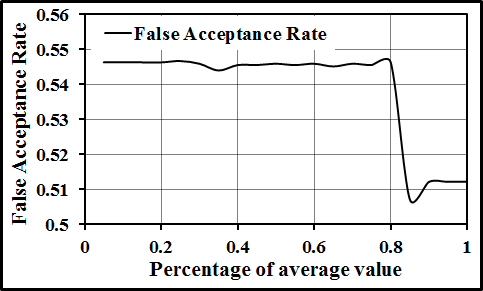
\includegraphics[width=2.5in,clip,keepaspectratio]{Chapters/figures/Emotion/lessDominant/fA}
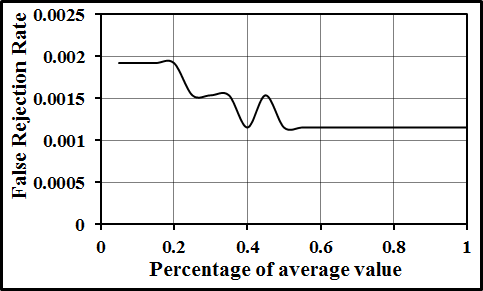
\includegraphics[width=2.5in,clip,keepaspectratio]{Chapters/figures/Emotion/lessDominant/fR}
\caption{percentage of average vs false accept rate and false reject rate in bounded k-means for less dominant emotion classification}
\label{Optional 6}
\end{figure}

\begin{figure}
\centering
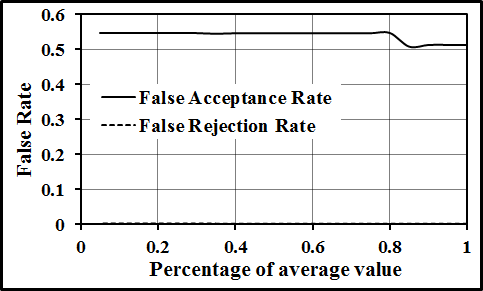
\includegraphics[width=4.25in,clip,keepaspectratio]{Chapters/figures/Emotion/lessDominant/fAfR}
\caption{percentage of average vs false accept rate and false reject rate in bounded k-means for less dominant emotion classification}
\label{Optional 6}
\end{figure}



\clearpage
\subsection{User classification}
\subsubsection{All user classification}
What about classifying a user based on his usage attributes. In this case we considered the data without any normalization. At first we tried to cluster the data with our unsupervised clustering approach (bounded k-means clustering). But we found it difficult to successfully identify users based on their usage attributes.
The experimental results are as follows


\subsubsection{Dominant user classification}
From matrix of users clusters, we found that some of the users heavily dominates others clusters. So we made an attempt to classify these dominant users. The results we found was much better than the general case. The results are illustrated below:

\begin{figure}
\centering
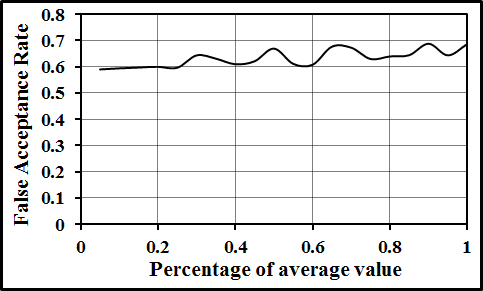
\includegraphics[width=2.5in,clip,keepaspectratio]{Chapters/figures/User/dominant/fA}
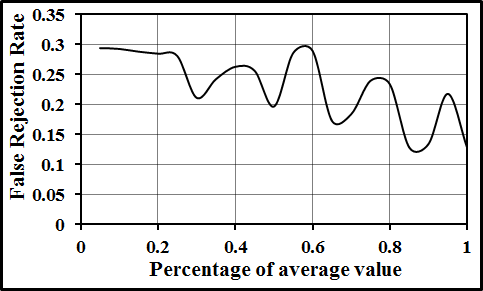
\includegraphics[width=2.5in,clip,keepaspectratio]{Chapters/figures/User/dominant/fR}
\caption{percentage of average vs false accept rate and false reject rate in bounded k-means for dominant user classification}
\label{Optional 6}
\end{figure}


\begin{figure}
\centering
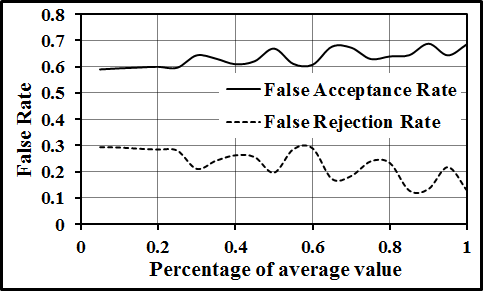
\includegraphics[width=4.25in,clip,keepaspectratio]{Chapters/figures/User/dominant/fAfR}
\caption{percentage of average vs both false acceptance rate and false rejection rate in bounded k-means for dominant user classification}
\label{Optional 6}
\end{figure}


\clearpage
\subsubsection{Dominant user classification with neutral emotion only}
From matrix of users clusters, we found that some of the users heavily dominates others clusters. So we made an attempt to classify these dominant users. The results we found was much better than the general case. The results are illustrated below:

\begin{figure}
\centering
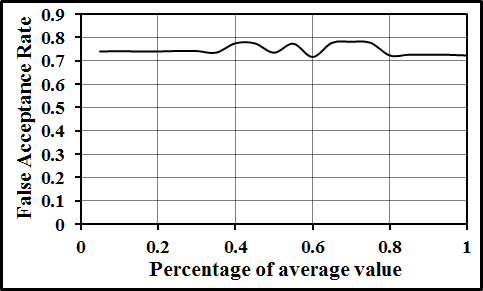
\includegraphics[width=2.5in,clip,keepaspectratio]{Chapters/figures/User/dominantWithNeutral/fA}
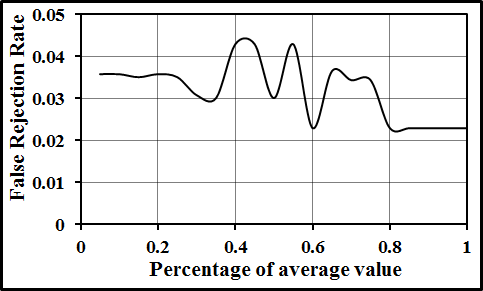
\includegraphics[width=2.5in,clip,keepaspectratio]{Chapters/figures/User/dominantWithNeutral/fR}
\caption{percentage of average vs false accept rate and false reject rate in bounded k-means for dominant user classification with neutral data only}
\label{Optional 6}
\end{figure}


\begin{figure}
\centering
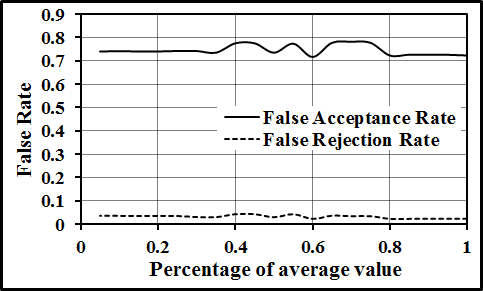
\includegraphics[width=4.25in,clip,keepaspectratio]{Chapters/figures/User/dominantWithNeutral/fAfR}

\caption{percentage of average vs false accept rate and false reject rate in bounded k-means for dominant user classification with neutral data only}
\label{Optional 6}
\end{figure}

\clearpage
\subsubsection{Less Dominant user classification with neutral emotion only}
From matrix of users clusters, we found that some of the users heavily dominates others clusters. So we made an attempt to classify these dominant users. The results we found was much better than the general case. The results are illustrated in figure 6.16.

\begin{figure}
\centering
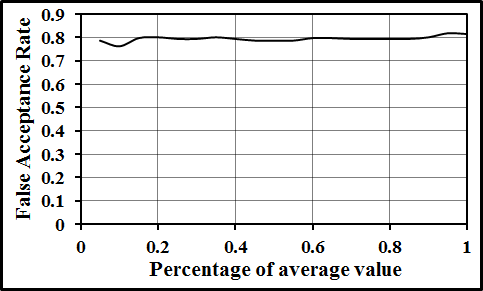
\includegraphics[width=2.5in,clip,keepaspectratio]{Chapters/figures/User/lessDominantWithNeutral/fA}
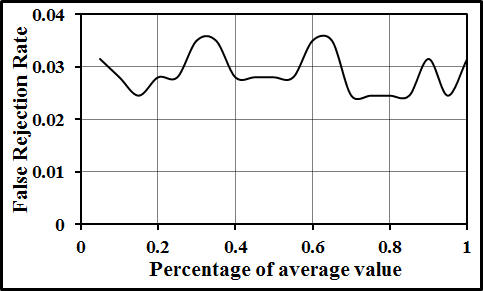
\includegraphics[width=2.5in,clip,keepaspectratio]{Chapters/figures/User/lessDominantWithNeutral/fR}
\caption{percentage of average vs false accept rate and false reject rate in bounded k-means for less dominant user classification with only neutral emotion's value}
\label{Optional 6}
\end{figure}

\begin{figure}
\centering
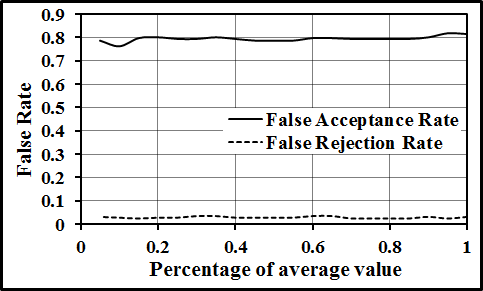
\includegraphics[width=4.25in,clip,keepaspectratio]{Chapters/figures/User/lessDominantWithNeutral/fAfR}
\caption{percentage of average vs false accept rate and false reject rate in bounded k-means for less dominant user classification with only neutral emotion's value}
\label{Optional 6}
\end{figure}




% Balancing columns in a ref list is a bit of a pain because you
% either use a hack like flushend or balance, or manually insert
% a column break.  http://www.tex.ac.uk/cgi-bin/texfaq2html?label=balance
% multicols doesn't work because we're already in two-column mode,
% and flushend isn't awesome, so I choose balance.  See this
% for more info: http://cs.brown.edu/system/software/latex/doc/balance.pdf
%
% Note that in a perfect world balance wants to be in the first
% column of the last page.
%
% If balance doesn't work for you, you can remove that and
% hard-code a column break into the bbl file right before you
% submit:
%
% http://stackoverflow.com/questions/2149854/how-to-manually-equalize-columns-
% in-an-ieee-paper-if-using-bibtex
%
% Or, just remove \balance and give up on balancing the last page.
%

